\chapter{Results and discussion}
\label{chap:results}
In this chapter, we present the results of our experiments.
When comparing tasks performance, we implicitly use F1 Macro as
all tasks but Day Of Week are imbalanced. We start with an overall
comparison of the models. We then do a closer analysis of the
individual tasks. Finally, we assess the overall performance
on tasks and put it into context with other works.

\section{Model Results}
\label{sec:results}
\begin{table}[h]
    \resizebox{\linewidth}{!}{%
        \centering\footnotesize\sf
        \begin{tabular}{lrrrrrrrr}
            \toprule
            {}    & \multicolumn{2}{l}{Server} & \multicolumn{2}{l}{Category} & \multicolumn{2}{l}{Gender} & \multicolumn{2}{l}{Day of week}                                                                     \\
            {}    & F1-macro                   & F1-micro                     & F1-macro                   & F1-micro                        & F1-macro       & F1-micro       & F1-macro       & F1-micro       \\
            \midrule
            Human & 27.03                      & 30.25                        & 40.26                      & 60.76                           & 50.09          & 61.75          & 13.53          & 13.75          \\
            Final & \textbf{71.22}             & \textbf{80.00}               & \textbf{52.04}             & \textbf{79.59}                  & \textbf{52.79} & \textbf{79.00} & \textbf{28.37} & \textbf{29.00} \\
            \bottomrule
        \end{tabular}
        \caption{Results on Human Test set. We use bold to denote the best result for each task.}
        \label{tab:results-human}
    }
\end{table}

\subsection{Human agreement and Human Test set}
\label{sec:human-baseline}
We found the average Cohen's kappa to be: 0.08 for Server, 0.65 for Category,
0.20 for Gender and 0.01 for Day Of Week. Based on the classification from \autoref{sec:interannotator},
only the category task showed at least substantial agreement.

As for performance results (see~\autoref{tab:results-human}), we found that humans were far below the performance
of the Final model on most of the tasks.
This is especially true for Server task, where the Final model beat Human by over 44 percent.
The only task where the Human was competitive is Gender, as the difference was just 2 percent.


\begin{table}[h]
    \resizebox{\linewidth}{!}{%
        \centering\footnotesize\sf
        \begin{tabular}{lrrrrrrrr}
            \toprule
            {}       & \multicolumn{2}{l}{Server} & \multicolumn{2}{l}{Category} & \multicolumn{2}{l}{Gender} & \multicolumn{2}{l}{Day of week}                                                                     \\
            {}       & F1-macro                   & F1-micro                     & F1-macro                   & F1-micro                        & F1-macro       & F1-micro       & F1-macro       & F1-micro       \\
            \midrule
            LR-50    & 36.92                      & 52.78                        & 33.30                      & 72.32                           & 43.62          & 69.15          & 18.13          & 19.62          \\
            LR-200   & 37.27                      & 53.38                        & 32.77                      & 72.69                           & 44.06          & 69.83          & 18.34          & 19.97          \\
            \addlinespace
            R-Base   & 69.74                      & 78.19                        & 54.35                      & 79.67                           & 51.18          & 74.67          & 29.43          & 29.49          \\
            F-Base   & 69.39                      & 77.68                        & 53.97                      & 79.55                           & -              & -              & 29.24          & 29.34          \\
            R-Short  & 59.48                      & 67.85                        & 36.55                      & 77.46                           & 44.97          & 69.95          & 17.42          & 19.61          \\
            \addlinespace
            Truncate & 68.71                      & 77.31                        & 53.90                      & 79.37                           & 50.36          & 74.21          & 29.52          & 29.57          \\
            LM-tune  & 70.06                      & 78.40                        & 55.18                      & 80.14                           & 51.13          & \textbf{75.09} & \textbf{29.98} & \textbf{30.00} \\
            Grad-12  & 67.81                      & 76.36                        & 51.93                      & 78.69                           & 49.98          & 73.82          & 29.11          & 29.21          \\
            Grad-24  & 69.07                      & 77.69                        & 53.22                      & 78.97                           & 49.75          & 74.06          & 29.36          & 29.47          \\
            \addlinespace
            Final    & \textbf{71.04}             & \textbf{79.25}               & \textbf{56.06}             & \textbf{80.47}                  & \textbf{51.94} & 75.04          & 29.68          & 29.69          \\
            \bottomrule
        \end{tabular}
        \caption{Results on Test set. We use bold to denote the best result for each task}
        \label{tab:results-test}
    }
\end{table}

\subsection{Baseline model}
\label{sec:baseline}
The baseline model results are shown in \autoref{tab:results-test}.
We have observed a tiny improvement by adding the additional 150k features.
We also inspected the features with the highest weights for each task and class, which
can be seen in \autoref{ch:baseline_features}.


\subsection{Backbone models}
As for backbone models, we found R-Base to outperform F-Base on all tasks by a small margin.
As noted in \autoref{sec:backbone}, the F-Base was very sensitive to the higher learning rate.
That's why the results are empty for Gender, as it diverged with every \ac{lr} we tried.
\begin{table}[h]
    \resizebox{\linewidth}{!}{%
        \centering\footnotesize\sf
        \begin{tabular}{lrrrrrrrr}
            \toprule
            {}      & \multicolumn{2}{l}{Server} & \multicolumn{2}{l}{Category} & \multicolumn{2}{l}{Gender} & \multicolumn{2}{l}{Day of week}                                                                     \\
            {}      & F1-macro                   & F1-micro                     & F1-macro                   & F1-micro                        & F1-macro       & F1-micro       & F1-macro       & F1-micro       \\
            \midrule
            R-Base  & \textbf{78.43}             & \textbf{82.88}               & \textbf{56.17}             & \textbf{80.65}                  & \textbf{52.38} & \textbf{75.61} & \textbf{27.96} & \textbf{28.33} \\
            \addlinespace
            R-Short & 75.12                      & 80.37                        & 37.88                      & 77.69                           & 47.45          & 74.30          & 17.41          & 19.82          \\
            F-Short & -                          & -                            & 39.31                      & 77.88                           & -              & -              & 17.68          & 19.20          \\
            GPT-3   & 67.30                      & 73.12                        & 44.76                      & 75.21                           & 42.92          & 70.28          & 19.49          & 20.83          \\
            \bottomrule
        \end{tabular}
        \caption{Results on Test Small. We use bold to denote the best result for each task}
        \label{tab:results-small}
    }
\end{table}

The Short train setting yielded opposite results as seen in \autoref{tab:results-small}.
For every task where F-Short hasn't diverged, it outperformed R-Short.
We believe that the dominance of Fernet-News in the Short setting is due to
better weights initialization, as the domain of the data is the same
in case of Fernet-News unlike in RobeCzech.
When trained in a full setting, initial weight becomes less relevant and the essential
factor is the slightly bigger capacity of RobeCzech. We also observed
higher \ac{achpt} at RobeCzech than Fernet-News: 4.68 vs 4.46.
This means that RobeCzech observes a slightly bigger portion of articles on average.

As for GPT-3, we found it to outperform both Short models on Category and Day of Week.
Since the model is multi-lingual and was trained in multi-task purely generative setting,
it's a great result. Due to its multi-linguality, we found CHpT to be just
1.77, which made the fine-tuning more expensive than expected.
Overall we spend around 40\$ for both training and inference.

We were surprised by the good performances of the Short models on Test Small set.
Especially in the case of Gender and Server, the performances were comparable with model R-Base, while
training on less than 6\% of the data. However, when we tested the R-Short on the Full Test set,
we found a more significant performance drop.

\subsection{Fine-tuning}
\begin{figure}[ht]
    \centering
    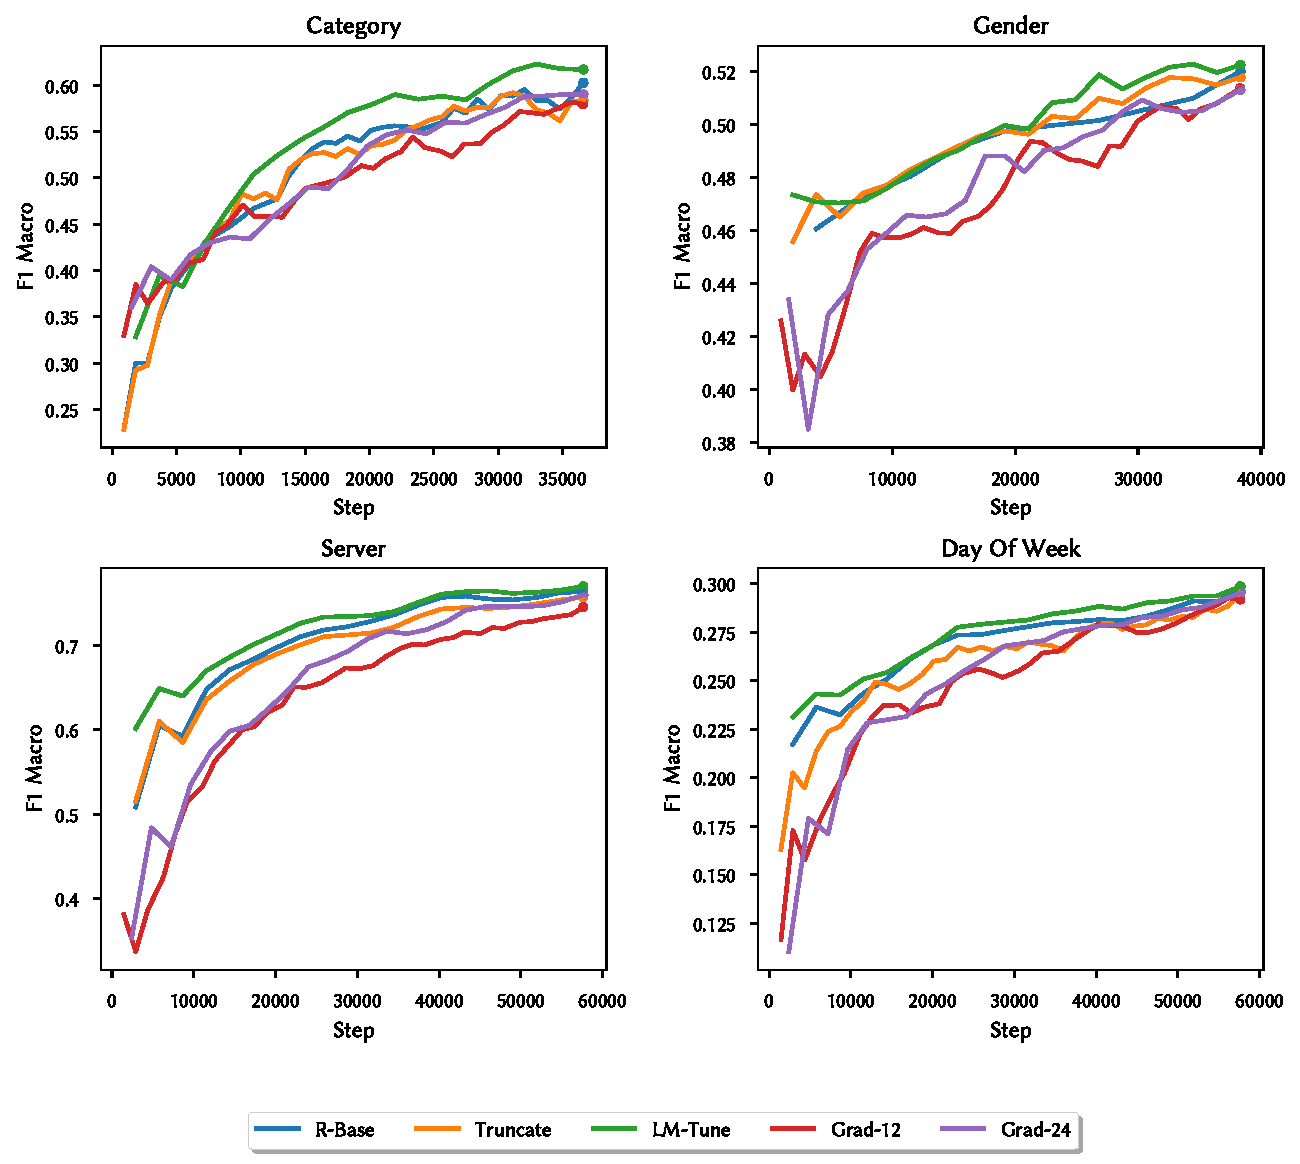
\includegraphics[width=1.0\textwidth]{graph_create/outputs/tune.pdf}
    \caption{Validation curves for all tasks of fine-tuning approaches. The curves are displayed
        with linear smoothing. Each Validation was run on 10\% of the Validation set. The last validation
        was run on the whole Validation set.}
    \label{fig:vallidation-curves-tune}
\end{figure}
Different truncations didn't help with performance, as seen at~\autoref{fig:vallidation-curves-tune}.
The same was observed with \ac{gu}, which even significantly worsened the performance
in some cases. From validation curves, we can observe that on all tasks but Category,
\ac{gu} performance falls behind considerably at the beginning of the training and
catches up only at the end for all but category tasks.
We think that's because Category can highly leverage the intrinsic values
occurring in lower layers of the transformer and just a slight modification of weight is needed,
while in other tasks, further training of lower layers is needed, and thus
\ac{gu} falls behind, as the layers are frozen at the start.

The only positive aspect we found with \ac{gu} was that it enabled us to have a higher batch
size on GPU, which sped up the training slightly.
Out of all fine-tuning approaches, only \ac{flm} increased performance.

\subsection{Final model}
\label{sec:final-model-performance-on-tasks}
We observe that further enhancements of the model improved the performance.
The only task where the Final model didn't outperform others was Day of Week.

\section{Tasks Inspection}
We decided to use the Final model for in-depth evaluation of all tasks, even
though it wasn't the best performing model for Day Of Week.


\subsubsection{Server}
\label{sec:final-model-performance-on-server}
\begin{table}[H]
    \centering\footnotesize\sf
    \begin{tabular}{lrrr}
        \toprule
        {}              & Precision & Recall & F1    \\
        \midrule
        SeznamZprávy.cz & 82.44     & 65.06  & 72.72 \\
        iDNES.cz        & 68.56     & 75.60  & 71.91 \\
        Aktuálně.cz     & 83.08     & 81.30  & 82.18 \\
        Novinky.cz      & 29.64     & 67.75  & 41.23 \\
        Deník.cz        & 91.75     & 86.39  & 88.99 \\
        iRozhlas.cz     & 60.43     & 80.95  & 69.20 \\
        Macro Avg       & 69.32     & 76.17  & 71.04 \\
        \bottomrule
    \end{tabular}
    \caption{Classification report of Server on Test set.}
    \label{tab:classification-report-server}
\end{table}
For Server, we observed the most problematic origin to be Novinky.cz. The model
incurs a significant precision drop on this origin as seen in \autoref{tab:classification-report-server}.
We assume this is due to distribution changes in Train and Test set.
Test set has very few samples of Novinky.cz, compared to the training set.
Overpredicting Novinky.cz is then natural behavior.

The opposite can be observed with
SeznamZprávy.cz. The model underpredicts this origin which results in low
recall. This can also be observed at~\autoref{fig:server-conf} as SeznamZprávy.cz is
often misclassified as Idnes.cz.

\subsubsection{Category}
\label{sec:final-model-performance-on-category}
\begin{table}[H]
    \centering\footnotesize\sf
    \begin{tabular}{lrrr}
        \toprule
        {}                     & Precision & Recall & F1    \\
        \midrule
        World                  & 82.62     & 86.77  & 84.65 \\
        Home                   & 86.89     & 82.91  & 84.86 \\
        Sport                  & 97.78     & 97.97  & 97.87 \\
        Culture                & 58.07     & 87.26  & 69.73 \\
        Celebrity              & 81.91     & 67.78  & 74.18 \\
        Gossip and Curiosities & 28.08     & 45.34  & 34.68 \\
        Economics              & 51.35     & 65.99  & 57.76 \\
        Crime                  & 60.58     & 62.30  & 61.43 \\
        Entrepreneurship       & 28.68     & 51.80  & 36.92 \\
        Car                    & 85.45     & 86.31  & 85.88 \\
        Science                & 54.35     & 51.48  & 52.87 \\
        Comments               & 68.88     & 85.70  & 76.38 \\
        Travel                 & 36.83     & 39.55  & 38.14 \\
        Finance                & 60.21     & 59.44  & 59.82 \\
        Technology             & 79.76     & 82.70  & 81.20 \\
        Housing                & 67.56     & 75.69  & 71.39 \\
        Coronavirus            & 42.72     & 33.24  & 37.39 \\
        Business               & 62.78     & 51.72  & 56.71 \\
        Interviews             & 7.95      & 8.64   & 8.28  \\
        Podcasts               & 0.00      & 0.00   & 0.00  \\
        Lifestyle              & 53.12     & 46.00  & 49.30 \\
        Literature             & 90.24     & 82.68  & 86.30 \\
        Christmas              & 11.11     & 25.00  & 15.38 \\
        Fine Arts              & 92.19     & 71.08  & 80.27 \\
        Bicycle                & 0.00      & 0.00   & 0.00  \\
        Macro Avg              & 55.57     & 57.89  & 56.06 \\
        \bottomrule
    \end{tabular}
    \caption{Classification report of Category on Test set.}
    \label{tab:classification-report-category}
\end{table}
The Category showed to be the most problematic task. While we thought that
we made the boundaries of the categories clear, the model predictions
suggests opposite. For example as seen in~\autoref{fig:category-conf}
the model often misclassified Fine Arts and Literature as Culture.
This is understandable
as Culture can be seen as a broader category. Similar can be observed with
Business, Entrepreneurship and Finance mistook for Economy. Another problem
we can observe is Coronavirus being misclassified as Home. The problem
is that not all news sever have the category Coronavirus. As the often topic of
the Coronavirus is politics, they will mark the article as Home. The only category
with great performance is Sports. Unsurprisingly this category has quite
clear boundaries.
\subsubsection{Gender}
\begin{table}[H]
    \centering\footnotesize\sf
    \begin{tabular}{lrrr}
        \toprule
        {}        & Precision & Recall & F1    \\
        \midrule
        Man       & 82.70     & 78.73  & 80.67 \\
        Woman     & 63.79     & 72.22  & 67.75 \\
        Mixed     & 23.89     & 4.38   & 7.41  \\
        Macro Avg & 56.79     & 51.78  & 51.94 \\
        \bottomrule
    \end{tabular}
    \caption{Classification report of Gender on Test set.}
    \label{tab:classification-report-gender}
\end{table}
What is clear from both the confusion matrix~(\autoref{fig:gender-conf}) and \autoref{tab:classification-report-gender}.
is that the Mixed class is highly problematic for the model. We explain this by its
lower representation in data. When it comes to Man and Woman comparison,
we observed Woman to have both precision and recall smaller. While we expected
the recall to be smaller, due to imbalance, we didn't expect the precision to be
lower as well.

\subsubsection{Day of week}
\begin{table}[H]
    \centering\footnotesize\sf
    \begin{tabular}{lrrr}
        \toprule
        {}        & Precision & Recall & F1    \\
        \midrule
        Monday    & 30.08     & 34.02  & 31.93 \\
        Tuesday   & 27.69     & 28.23  & 27.95 \\
        Wednesday & 30.28     & 27.57  & 28.86 \\
        Thursday  & 25.45     & 34.57  & 29.32 \\
        Friday    & 33.22     & 28.60  & 30.73 \\
        Saturday  & 34.86     & 22.63  & 27.44 \\
        Sunday    & 33.95     & 29.37  & 31.49 \\
        Macro Avg & 30.79     & 29.28  & 29.68 \\
        \bottomrule
    \end{tabular}
    \caption{Classification report of Day Of Week on Test set.}
    \label{tab:classification-report-day}
\end{table}
From the confusion matrix~(\autoref{fig:day-conf}), we can see the model misclassifying the days
as surroundings of the target day. The only exception to this rule
is weekend days. This can be observed with both Monday and Friday, as they are
rather misclassified as random weekdays rather than surrounding Saturday, respectively
Sunday.



\subsection{Tasks in context}
\label{sec:tasks_in_context}

\subsection{Server and Day of Week}
As for Server and Day of Week tasks, we are unaware of any previous work.
Considering the terrible Human performance and agreement, we find both results
reasonable.

\subsubsection{Category}
The category has been researched quite well by works such as \cite{sunagar2021news} and \cite{fuksClassificationNewsDataset}.

In the first work, the authors report 90.85\% F1 Micro; however,
the authors only used four categories from a single source.

The second work is more comparable as the authors used the same number of categories (25) but from a single source.
The authors report 68.38\% F1 Micro. We thus find our results reasonably good. It's worth
noting that while F1 Macro looks very bad, the misclassifications often have
reasonable explanations. This points to the fact, that better metric should be used.

\subsubsection{Gender}
Gender task has also been studied in a few works such as \cite{haagsmaOverviewCrossGenreGender}
. The study is an overview of shared gender classification task in Dutch.
The data are gathered from multiple Dutch news sources but
don't consider multi-author articles. Authors report 68.9\% F1 Micro for the best model.
This makes our results look great. Note, however, that the language difference could play
a huge role.